\chapter{تخصیص منابع در حالت تقسیم زمانی دینامیکی در شبکه دسترسی رادیویی}
\section{مقدمه}
در این فصل هدف بدست آوردن مدل سیستم در حالت تقسیم زمانی یا \lr{TDD} \LTRfootnote{Time Division Duplexing} دینامیکی می باشد که بدین منظور تخصیص توان برای هر دو لینک فراسو و فروسو به طور همزمان بدست می آید.
در تقسیم زمانی دینامیکی، منابع به صورت دینامیکی بین هر دو لینک فراسو و فروسو  تخصیص داده می شود. در سیستم های سنتی  ایستگاه پایه و سیستم سنتی ایستگاه پایه و واحد رادیویی که در فصل اول بیان شد، تداخل بین لینک فراسو و فروسو منجر به کاهش شدید در بازدهی انرژی می گردد در حالی که در سیستم \lr{C-RAN} این تداخل  به دلیل وجود \lr{BBU Pool} و واحد های رادیویی \lr{RRH} و نوع پردازش هایی که در آنها صورت می گیرد، تاثیر چندانی در بازدهی انرژی نمی گذارد \cite{TDD,dynamic}.


حال در ادامه، مدل سیستمی با ساختار \lr{C-RAN}  بیان می نماییم که دارای چندین خوشه است که تعدادی از این خوشه  ها در لینک فراسو و تعدادی دیگر در لینک فروسو عمل می کنند. همچنین تمام واحدهای رادیویی در این خوشه ها به واحد کنترل ابری \lr{BBU Pool} از طریق لینک \lr{fronthaul} با ظرفیت محدود، متصلند. سیگنالهای خوشه های لینک فراسو و فروسو نیز بر یکدیگر تداخل اعمال می کنند.
\section{مدل سیستم}
در این بخش مدل سیستمی برای حالت تقسیم زمانی دینامیکی  براساس معماری \lr{C-RAN} در لینک فراسو و فروسو همانند فصل 3 بیان می شود. فرض بر این است که این سیستم شامل $S$ خوشه می باشد که $S_1$ خوشه در لینک فروسو و $S_2$
 خوشه در لینک فراسو عمل می کنند که :
 $S_1 + S_2 = S$
 است.
 همچنین هر خوشه ی $v$ دارای  $R_v$  واحد رادیویی و $D_v$ کاربر می باشد.  
 علاوه براین، فرض بر این است که
$j$
امین واحد رادیویی، در $v$امین خوشه، توسط لینک فیبر نوری با ظرفیت محدود $C_{r_{(v,j)}}$ به واحد کنترل متصل می گردد. در نتیجه داریم:
\begin{equation}
\begin{split}
\mathcal{R}_v= \{  r_{(v,i)} | 1 \leq i \leq {R}_v , i\in Z^+\}, \\
\mathcal{C}_{\mathcal{R}_v}= \{C_{r_{(v,j)}}| 1 \leq j \leq {R}_v , j\in Z^+\}, \\
\mathcal{D}_v= \{  d_{(v,k)} | 1 \leq k \leq {D}_v , k\in Z^+\},  \\
\end{split}
\end{equation} 
که
 $\mathcal{R}_v$، $\mathcal{C}_{\mathcal{R}_v}$
 و
  $\mathcal{D}_v$
 به ترتیب نشان دهنده ی دسته واحدهای رادیویی، دسته ی ظرفیت لینک \lr{Fronthaul} و دسته ی کاربران در $v$امین دسته ی خوشه می باشد.\newline
واحدهای رادیویی
 تداخل پیام ها را از خوشه های دیگر لینک فراسو و فروسو دریافت می کنند.
\newline
 \subsection{آنالیز نرخ قابل دسترس در خوشه های فروسو}
در این قسمت، هدف بررسی نرخ قابل دسترسی سیستم برای خوشه هایی است که در حال تبادل در لینک فروسو می باشند.
 نرخ قابل دسترسی برای کاربر $d_{(s,k)}$ به صورت زیر می باشد:
\begin{equation}\label{e1}
\mathfrak{R}_{d_{(s,k)}} = B \log_2(1+\gamma_{d_{(s,k)}}),
\end{equation}
که $B$ پهنای باند کانال و $\gamma_{d_{(s,k)}}$ همان \lr{SINR} دریافتی $k$امین کاربر در $s$امین دسته ی خوشه است که به صورت زیر بیان می گردد.  
\begin{equation}\label{51}
\gamma_{d_{(s,k)}}= \frac{p_{d_{(s,k)}}|\boldsymbol{h}_{\mathcal{R}_s, d_{(s,k)}}^H \boldsymbol{w}_{\mathcal{R}_{s},d_{(s,k)}}|^2}{I_{d_{(s,k)}}+BN_0}.
\end{equation}
در فرمول \eqref{51}، 
$I_{d_{(s,k)}}$
نشان دهنده ی توان سیگنال تداخلی است.$BN_0$
نشان دهنده ی توان نویز است و
$\boldsymbol{h}_{\mathcal{R}_s, d_{(s,k)}}$ 
 نشان دهنده ی بردار گین کانال بین $k$امین کاربر و واحدهای رادیویی
 $s$
 امین دسته ی خوشه در حالت لینک فروسو می باشد. همچنین 
 $\boldsymbol{w}_{\mathcal{R}_{s},d_{(s,k)}}$
 نشان دهنده ی بردار پیش کدگذاری استفاده شده در $s$امین دسته ی خوشه ها برای $k$امین کاربر می باشد. 
 $p_{d_{(s,k)}}$
 توان ارسالی واحدهای رادیویی است که به $k$امین کاربر در $s$امین دسته ی خوشه ارسال می گردد.


برای بدست آوردن  $\gamma_{d_{(s,k)}}$، ابتدا سیگنال دریافتی را نمایش می دهیم. سیگنال دریافتی لینک فروسو توسط کاربر $k$ ام در خوشه ی $s$ ام به این صورت نمایش داده می شود
\begin{equation}\label{6}
\begin{split}
y_{d_{(s,k)}} &= \underbrace{\sqrt{p_{d_{(s,k)}}}\boldsymbol{h}_{\mathcal{R}_s, d_{(s,k)}}^H \boldsymbol{w}_{\mathcal{R}_{s},d_{(s,k)}} x_{d_{(s,k)}} }_{\text{\lr{(desired signal)}}} + \underbrace{\sum_{\substack{l=1 \\ l\neq k}}^{{D}_s} \boldsymbol{h}_{\mathcal{R}_s, d_{(s,k)}}^H \boldsymbol{w}_{\mathcal{R}_{s},d_{(s,l)}}  \sqrt{p_{d_{(s,l)}}}  x_{d_{(s,l)}}}_{\text{(\lr{intra-cluster interference})}}\\
&+\underbrace{\sum_{\substack{v=1 \\ v\neq s}}^{S_1} \sum_{l=1}^{{D}_v} \boldsymbol{h}_{\mathcal{R}_v, d_{(s,k)}}^H \boldsymbol{w}_{\mathcal{R}_{v},d_{(v,l)}} 
\sqrt{p_{d_{(v,l)}}}  x_{d_{(v,l)}}}_{\text{(\lr{inter-cluster interference})}}+\underbrace{\sum_{\substack{t=1}}^{S_2} \sum_{l=1}^{{D}_t} \boldsymbol{b}_{\mathcal{D}_t, d_{(s,k)}}^H \sqrt{ p_{d_{(t,l)}}}  x_{d_{(t,l)}}}_{\text{(\lr{ interference from uplink's clusters})}}  \\
& +\underbrace{ \sum_{v=1}^{S_1} \sum_{i=1}^{{R}_v} q_{r_{(v,i)}} h_{r_{(v,i)}, d_{(s,k)}} }_{\text{(\lr{quantization noise interference})}}+ z_{d_{(s,k)}} .\\
\end{split}
\end{equation}
که در اینجا،
 $\boldsymbol{b}_{\mathcal{D}_t, d_{(s,k)}}  \in \mathbb{C}^{\mathcal{D}_t\times 1}$
 ، بردار کانال بین کاربران لینک فراسو در خوشه ی $t$ ام به $k$امین کاربر لینک فروسو در خوشه ی   $s$
 ام 
می باشد که همانند پارامتر بردار کانال $h$ بدست می آید. بقیه ی پارامترها نیز در فصل 3 به طور کامل بیان شده است.\\
با توجه به \eqref{6}، 
$I_{d_{(s,k)}}$ 
از رابطه ی زیر  بدست می آید.
\begin{equation}\label{7}
\begin{split}
I_{d_{(s,k)}} &=  \underbrace{\sum_{\substack{l=1 \\ l\neq k}}^{{D}_s} |\boldsymbol{h}_{\mathcal{R}_s, d_{(s,k)}}^H \boldsymbol{w}_{\mathcal{R}_{s},d_{(s,l)}}|^2  p_{d_{(s,l)}}}_{\text{(\lr{intra-cluster interference})}}
+\underbrace{\sum_{\substack{v=1 \\ v\neq s}}^{S_1} \sum_{l=1}^{{D}_v} |\boldsymbol{h}_{\mathcal{R}_v, d_{(s,k)}}^H \boldsymbol{w}_{\mathcal{R}_{v},d_{(v,l)}}|^2 p_{d_{(v,l)}}}_{\text{(\lr{inter-cluster interference})}}\\
&+\underbrace{\sum_{\substack{t=1}}^{S_2} \sum_{l=1}^{{D}_t} |\boldsymbol{b}_{\mathcal{D}_t, d_{(s,k)}}^H|^2  p_{d_{(t,l)}}}_{\text{(\lr{ interference from uplink's clusters})}} 
 +\underbrace{ \sum_{v=1}^{S_1} \sum_{i=1}^{{R}_v} {\sigma_q}_{r_{(v,i)}}^2  |h_{r_{(v,i)}, d_{(s,k)}}|^2 }_{\text{(\lr{quantization noise interference})}}.
\end{split}
\end{equation}
  همچنین توان سیگنال ارسالی به این صورت بدست می آید
\begin{equation}
\bar{p}_{r_{(s,i)}} = \boldsymbol{w}_{r_{(s,i)},\mathcal{D}_{s}} \boldsymbol{P}_{\mathcal{D}_s}^{\frac{1}{2}} \boldsymbol{P}_{\mathcal{D}_s}^{H \frac{1}{2}}   \boldsymbol{w}_{r_{(s,i)},\mathcal{D}_{s}}^H + \sigma_{q_{(s,i)}}^2 .
\end{equation}
و داریم:
\begin{equation}
P_{dl}= \sum_{s=1}^{S_1}\sum_{i=1}^{R_s}\bar{p}_{r_{(s,i)}} + P_c^{total,DL}
\end{equation}
که $ P_c^{total,DL}$، توان مداری کل واحدهای رادیویی لینک فروسو است.
در نتیجه نرخ قابل دسترس بر روی لینک \lr{fronthaul}، بین واحد کنترل و $i$امین واحد رادیویی در $t$امین خوشه  به صورت زیر بدست می آید 
\begin{equation}
C_{r_{(t,i)}} = \log{(1+\frac{w_{r_{(s,i)},\mathcal{D}_{s}} \boldsymbol{P}_{\mathcal{D}_s}^{\frac{1}{2}} \boldsymbol{P}_{\mathcal{D}_s}^{H \frac{1}{2}}   \boldsymbol{w}_{r_{(s,i)},\mathcal{D}_{s}}^H }{ \sigma_{q_{(s,i)}}^2})},
\end{equation}
 \subsection{آنالیز نرخ قابل دسترس در خوشه های فراسو}
 حال در این قسمت، هدف بررسی نرخ قابل دسترسی سیستم برای خوشه هایی است که در حال تبادل در لینک فراسو می باشند که همانند بخش قبلی بدست می آید.
 نرخ قابل دسترسی برای کاربر $d_{(s,k)}$ به این صورت است
\begin{equation}\label{e1}
\mathfrak{R}_{d_{(s,k)}} = B \log_2(1+\gamma_{d_{(s,k)}}),
\end{equation}
که $B$ پهنای باند کانال و $\gamma_{d_{(s,k)}}$ همان \lr{SINR} دریافتی $k$امین کاربر در $s$امین دسته ی خوشه است که در رابطه ی \eqref{5} آمده است.
\begin{equation}\label{5}
\gamma_{d_{(s,k)}}= \frac{p_{d_{(s,k)}} |{\boldsymbol{w}^H}_{\mathcal{R}_{s},d_{(s,k)}}^آ\boldsymbol{h}_{\mathcal{R}_s, d_{(s,k)}}|^2}{I_{d_{(s,k)}}+B\nu}.
\end{equation}
در فرمول \eqref{5}، 
$I_{d_{(s,k)}}$
نشان دهنده ی توان سیگنال تداخلی است.$B\nu$
نشان دهنده ی توان نویز است و
$\boldsymbol{h}_{\mathcal{R}_s, d_{(s,k)}}$ 
 نشان دهنده ی بردار کانال بین $k$امین کاربر و واحدهای رادیویی
 $s$
 امین دسته ی خوشه می باشد. همچنین 
 $\boldsymbol{w}_{\mathcal{R}_{s},d_{(s,k)}}$
 نشان دهنده ی بردار پرتو دهی استفاده شده در $s$امین دسته ی خوشه ها برروی واحدهای رادیویی برای بدست آوردن پیام $k$امین کاربر می باشد. 
 $p_{d_{(s,k)}}$
 توان ارسالی$k$امین کاربر در $s$امین دسته ی خوشه می باشد.
 در این قسمت می خواهیم $\gamma$ را بدست آوریم

پیام دریافتی توسط واحد رادیویی  $n$ ام در دسته ی $s$ ام در رابطه ی \eqref{100} نوشته شده است.
 \begin{equation} \label{100}
\begin{split}
y_{r_{(s,n)}} &=  \underbrace{ \sum_{k=1}^{D_s} h_{r_{(s,n)},d_{(s,k)}} \sqrt{p_{d_{(s,k)}}}  x_{d_{(s,k)}} }_{\text{\lr{desired signal}}}
+ \underbrace{\sum_{t=1,t\neq s}^{S_2} \sum_{j=1}^{D_t} h_{r_{(s,n)},d_{(t,j)}} \sqrt{p_{d_{(t,j)}}} x_{d_{(t,j)}}}_{\text{\lr{inter-cluster interference}}}\\
&+ \underbrace{\sum_{v=1}^{S_1}  \boldsymbol{f}_{\mathcal{R}_v, r_{(s,n)}}^H  \boldsymbol{W}_{\mathcal{R}_v,\mathcal{D}_v}^{DL} \boldsymbol{P}_{\mathcal{D}_v}^{1/2}  \boldsymbol{x}_{\mathcal{D}_v}}_{\text{\lr{downlink's cluster interference}}}
 + \underbrace{\boldsymbol{z}_{r_{(s,n)}}}_{\text{\lr{guassian noise}}}
 \end{split}
\end{equation}
که در اینجا $\boldsymbol{W}^{DL}$ ماتریس پیش کدگذاری در لینک فروسو می باشد.\\
پیام دریافتی توسط واحد رادیویی، بعد از فشرده سازی به صورت زیر می شود
\begin{equation}
\hat{y}_{r_{(s,n)}} = y_{r_{(s,n)}} + q_{r_{(s,n)}} 
\end{equation}
پیام هر کاربر در واحد کنترل با اعمال پرتو دهی \LTRfootnote{beamforming} به صورتی که در ادامه بیان شده، بدست می آید
%\begin{equation}
%\begin{split}
%\hat{x}_{d_{(s,k)}} = & {\boldsymbol{W}^H}_{\mathcal{R}_s, d_{(s,k)}} \boldsymbol{h}_{\mathcal{R}_s, d_{(s,k)}} \sqrt{p_{d_{(s,k)}}}  x_{d_{(s,k)}} \\
%+ & \sum_{i=1,i\neq k}^{K_s}  {\boldsymbol{W}^H}_{\mathcal{R}_s, d_{(s,k)}} \boldsymbol{h}_{\mathcal{R}_s, d_{(s,i)}} \sqrt{p_{d_{(s,i)}}}  x_{d_{(s,i)}} \\
%+&  \sum_{t=1,t\neq s}^{S} \sum_{j=1}^{K_t} {\boldsymbol{W}^H}_{\mathcal{R}_s, d_{(s,k)}} \boldsymbol{h}_{\mathcal{R}_s, d_{(t,j)}} \sqrt{p_{d_{(t,j)}}}  x_{d_{(t,j)}} \\
%+& {\boldsymbol{W}^H}_{\mathcal{R}_s, d_{(s,k)}}  ({\boldsymbol{q}}_{\mathcal{R}_s} + {\boldsymbol{z}}_{\mathcal{R}_s})
%\end{split}
%\end{equation}
\begin{equation}
\begin{split}
\hat{x}_{d_{(s,k)}} = &  \underbrace{ {\boldsymbol{w}^H}_{\mathcal{R}_s, d_{(s,k)}} \boldsymbol{h}_{\mathcal{R}_s, d_{(s,k)}} \sqrt{p_{d_{(s,k)}}}  x_{d_{(s,k)}}}_{\text{\lr{desired signal}}} 
+  \underbrace{ \sum_{i=1,i\neq k}^{D_s}  {\boldsymbol{w}^H}_{\mathcal{R}_s, d_{(s,k)}} \boldsymbol{h}_{\mathcal{R}_s, d_{(s,i)}} \sqrt{p_{d_{(s,i)}}}  x_{d_{(s,i)}}}_{\text{\lr{intra-cluster interference}}} \\
+&   \underbrace{ \sum_{t=1,t\neq s}^{S_2} \sum_{j=1}^{D_t} {\boldsymbol{w}^H}_{\mathcal{R}_s, d_{(s,k)}} \boldsymbol{h}_{\mathcal{R}_s, d_{(t,j)}} \sqrt{p_{d_{(t,j)}}}  x_{d_{(t,j)}}}_{\text{\lr{inter-cluster interference}}} 
+ \underbrace{\sum_{v=1}^{S_1} {\boldsymbol{w}^H}_{\mathcal{R}_s, d_{(s,k)}}    \boldsymbol{f}_{\mathcal{R}_v, \mathcal{R}_s}^H  \boldsymbol{W}_{\mathcal{R}_v,\mathcal{D}_v}^{DL} \boldsymbol{P}_{\mathcal{D}_v}^{1/2}  \boldsymbol{x}_{\mathcal{D}_v}}_{\text{\lr{downlink's cluster interference}}}\\
+& {\boldsymbol{w}^H}_{\mathcal{R}_s, d_{(s,k)}}  ({\boldsymbol{q}}_{\mathcal{R}_s} + {\boldsymbol{z}}_{\mathcal{R}_s})
\end{split}
\end{equation}
حال برای بدست آوردن \lr{SNR}، توان سیگنال بر روی توان تداخل و نویز مورد محاسبه قرار می گیرد.
\begin{equation}
\gamma = \frac{p_{d_{(s,k)}}|{\boldsymbol{W}^H}_{\mathcal{R}_s, d_{(s,k)}} \boldsymbol{h}_{\mathcal{R}_s, d_{(s,k)}}|^2}{
  I_{d_{(s,k)}}
+ B \times \nu_{d_{(s,k)}}
}
\end{equation}
همچنین می توان نوشت
\begin{equation}
\begin{split}
\nu_{d_{(s,k)}}&  = {\boldsymbol{w}^H}_{\mathcal{R}_s, d_{(s,k)}}  (diag(\sigma_n{r_{(s,1)}}^2...\sigma_n{r_{(s,R_s)}}^2)+diag(\sigma_q{r_{(s,1)}}^2...\sigma_q{r_{(s,R_s)}}^2)) {\boldsymbol{W}}_{\mathcal{R}_s, d_{(s,k)}}\\
I_{d_{(s,k)}}& = \sum_{i=1,i\neq k}^{D_s}  |{\boldsymbol{w}^H}_{\mathcal{R}_s, d_{(s,k)}} \boldsymbol{h}_{\mathcal{R}_s, d_{(s,i)}}|^2 p_{d_{(s,i)}} +\sum_{t=1,t\neq s}^{S_2} \sum_{j=1}^{D_t} |{\boldsymbol{w}^H}_{\mathcal{R}_s, d_{(s,k)}} \boldsymbol{h}_{\mathcal{R}_s, d_{(t,j)}}|^2 p_{d_{(t,j)}}+I_{d_{(s,k)}}^{dl} \\
\end{split}
\end{equation}
 در اینجا  $\sigma_n^2$ واریانس نویز می باشد که برای سادگی برای همه ی واحدهای رادیویی ثابت فرض شده و دارای مقدار $N_0$ 
است و $\sigma_q^2$ واریانس نویز فشرده سازی می باشد.
علاوه بر این، 
\begin{equation}
I_{d_{(s,k)}}^{dl} =   \sum_{v=1}^{S_1} || {\boldsymbol{w}^H}_{\mathcal{R}_s, d_{(s,k)}}  \boldsymbol{f}_{\mathcal{R}_v, \mathcal{R}_s}^H  \boldsymbol{W}_{\mathcal{R}_v,\mathcal{D}_v}^{DL} \boldsymbol{P}_{\mathcal{D}_v}^{1/2}||^2.
\end{equation}
می دانیم نرخ قابل دسترس بر روی لینک \lr{fronthaul}، بین $n$ امین واحد رادیویی در $s$ امین خوشه و واحد کنترل به صورت مقابل بدست می آید 
\begin{equation}
C_{r_{(s,n)}} = \log{\frac{( \sum_{k=1}^{D_t}|h_{r_{(s,n)},d_{(s,k)}}|^2{p_{d_{(s,k)}}}+ B N_0) }{ \sigma_{q_{(s,n)}}^2})},
\end{equation}
و کل توان لینک فراسو به این صورت است
\begin{equation}
P_{ul}= \sum_{s=1}^{S_2}\sum_{k=1}^{D_s}{p}_{d_{(s,k)}} + P_c^{total,UL}.
\end{equation}
که $ P_c^{total,UL}$، توان مداری کل واحدهای رادیویی لینک فراسو است.
\subsection{شرح مسئله}
 در اینحا  نسبت مجموع وزن دار نرخ ها لینک فروسو و فراسو در سیستم به مجموع وزن دار توان ارسالی بیشینه می گردد
که بیشینه سازی با شروط زیر مورد بررسی قرار می گیرد. 
\begin{equation}\label{p4}
\begin{aligned}
\max\limits_{\boldsymbol{P}}   \quad &  \tau= \frac{\sum\limits_{s=1}^{S_1} \sum\limits_{k=1}^{{D}_s}\mathfrak{R}_{d_{(s,k)}}^{DL} + \alpha \sum\limits_{s=1}^{S_2} \sum\limits_{k=1}^{{D}_s}\mathfrak{R}_{d_{(s,k)}}^{UL}} {P_{dll}+ \beta P_{ulL}}\\
\text{\lr{subject to}} \quad  & \bar{p}_{r_{(s,i)}} \leq P_{max}^{dl} && \qquad \forall s \in S_1, \forall i,   \\
&\mathfrak{R}_{d_{(s,k)}} \geq  \mathfrak{R}_{d_{(s,k)}}^{th} && \qquad \forall s, \forall k, \\
&C_{r_{(s,i)}} \leq C_{r_{(s,i)}}^{th}  &&\qquad \forall s, \forall i, \\
&p_{d_{(s,k)}}  \geq 0                                  &&\qquad \forall s, \forall k, \\
&p_{d_{(s,k)}}  \leq P_{max}^{ul}                                  &&\qquad \forall s, \forall k, \\
\end{aligned}			
\end{equation}
که در اینجا  $ \boldsymbol{P} = \{ \boldsymbol{P}_{\mathcal{D}_s}|  1 \leq s \leq S, s \in \mathbb{Z}^{+} \}$ ماتریس تخصیص توان است.
از آنجایی که این یک مسئله ی محدب نیست، با روش الگوریتم تکرار شونده ، مقدار توان بهینه بدست می آید\cite{boyd}.
\subsection{روش مورد استفاده}
در این قسمت، به جای بیشینه سازی $\tau$، مسئله ی معادل آن را با الگوریتم تکرار شونده حل می شود
\begin{theorem}\label{t2}
مقدار ماکسیمم $\tau^*$  تنها زمانی بدست می آید که
\begin{equation}\label{q2}
\begin{split}
&\max \limits_{\boldsymbol{P}} (\sum\limits_{s=1}^{S_1} \sum\limits_{k=1}^{{D}_s}\mathfrak{R}_{d_{(s,k)}}^{DL} + \alpha \sum\limits_{s=1}^{S_2} \sum\limits_{k=1}^{{D}_s}\mathfrak{R}_{d_{(s,k)}}^{UL}) - \tau^*(P_{dll}+ \beta P_{ulL} )=\\
& \sum\limits_{s=1}^{S_1} \sum\limits_{k=1}^{{D}_s}\mathfrak{R}_{d_{(s,k)}}^{*DL} + \alpha \sum\limits_{s=1}^{S_2} \sum\limits_{k=1}^{{D}_s}\mathfrak{R}_{d_{(s,k)}}^{*UL}) - \tau^*(P_{dll}^{*}+ \beta P_{ulL}^{*} )=0,
\end{split}
\end{equation}
که $\{\boldsymbol{P}\}$  یک پاسخ امکان پذیر برای مسئله ی \eqref{p1} باشد 
\cite{hcranEE}.
\end{theorem}
\begin{proof}
اثبات این قضیه با روش مشابه در مقاله ی \cite{hcranEE} حل شده است.
\end{proof}
این مسئله برای حل، به دو بخش مجزای بیشینه سازی برای لینک فروسو و فراسو تقسیم می گردد سپس دو بخش جدا شده با الگوریتم های تکرار شونده با یکدیگر حل می شوند و جواب بهینه را می دهند.
\subsection{الگوریتم لینک فروسو}
برای حل مسئله ی بهینه سازی لینک فروسو، از تابع لاگرانژ استفاده می کنیم \cite{boyd} که توسط الگوریتم تکرار شونده بدست می آید. 
الگوریتم تکرار شونده برای بهینه سازی مورد استفاده قرار می گیرد که براساس ضرایب تابع لاگرانژ می باشد 
\begin{equation}
\begin{split}
\mathcal{L}(\boldsymbol{P}; \boldsymbol{\lambda}, \boldsymbol{\mu}, \boldsymbol{ \kappa}) & = \sum\limits_{s=1}^{S_1} \sum\limits_{k=1}^{\mathcal{D}_s}\mathfrak{\tilde{R}}_{d_{(s,k)}} 
- \eta \sum\limits_{s=1}^{S_1} \sum\limits_{i=1}^{\mathcal{R}_s}\bar{p}_{r_{(s,i)}} - \eta P_c^{total, dl}\\
&+\sum\limits_{s=1}^{S_1} \sum\limits_{k=1}^{\mathcal{D}_s} \lambda_{d_{(s,k)}} (\mathfrak{\tilde{R}}_{d_{(s,k)}}-\mathfrak{R}_{d_{(s,k)}}^{th})\\
&- \sum\limits_{s=1}^{S_1} \sum\limits_{i=1}^{\mathcal{R}_s} \mu_{r_{(s,i)}} (\bar{p}_{r_{(s,i)}}-P_{max})\\
&- \sum\limits_{s=1}^{S_1} \sum\limits_{i=1}^{\mathcal{R}_s} \kappa_{r_{(s,i)}} (C_{r_{(s,i)}}-C_{r_{(s,i)}}^{th}).\\
\end{split}
\end{equation}
که در اینجا، $\boldsymbol{\lambda}, \boldsymbol{\mu}, \boldsymbol{\kappa} \geq 0$
بردارهای ضرایب لاگرانژ می باشد .\newline
همچنین برای ساده سازی می توان نوشت:
\begin{equation}
\begin{split}
\tilde{I}_{d_{(s,k)}} &= \sum_{v=1}^{S_1} P_{max}|| \boldsymbol{h}_{\mathcal{R}_v,d_{(s,k)}} \boldsymbol{w}_{\mathcal{R}_v,d_{(s,k)}}||^2  +  \sum_{v=1}^{S} \sum_{i=1}^{{R}_v} {\sigma_q}_{r_{(v,i)}}^2  |h_{r_{(v,i)}, d_{(s,k)}}|^2 \\
&+ \sum_{\substack{t=1}}^{S_2} \sum_{l=1}^{{D}_t} |\boldsymbol{b}_{\mathcal{D}_t, d_{(s,k)}}^H|^2  p_{d_{(t,l)}}.
\end{split}
\end{equation}
با استفاده از این معادله، توان بهینه به صورت مقابل بدست می آید
\begin{equation}
p_{d_{(s,k)}}^* =[\frac{ B(1+\lambda_{d_{(s,k)}} )}{\ln2 \times (\iota_{d_{(s,k)}}+ \chi_{d_{(s,k)}})} -\frac{\tilde{I}_{d_{(s,k)}} + BN_0}{\nu_{d_{(s,k)}} }]^+;
\end{equation} 
که 
 $$\nu_{d_{(s,k)}} =|h_{\mathcal{R}_s, d_{(s,k)}}^H \boldsymbol{w}_{R_{s},d_{(s,k)}}|^2,$$
 $$\iota_{d_{(s,k)}}= \sum\limits_{i=1}^{\mathcal{R}_s} (\mu_{r_{(s,i)}}+\eta)(w_{r_{(s,i)},d_{(s,k)}} w_{r_{(s,i)},d_{(s,k)}}^*),$$
 $$\chi_{r_{(s,i)}} \approx  \sum\limits_{i=1}^{\mathcal{R}_s} \frac{\kappa_{r_{(s,i)}}}{\ln 2}\frac{(w_{r_{(s,i)},d_{(s,k)}} w_{r_{(s,i)},d_{(s,k)}}^*)}{ P_{max}}.$$
\subsection{الگوریتم لینک فراسو}
 ابتدا کران بالایی برای تداخل بدست می آید که در ادامه بیان می شود.
\begin{equation} \label{id}
\tilde{I}_{d_{(s,k)}} = \sum_{v=1}^{S_2}  |{\boldsymbol{w}^H}_{\mathcal{R}_s, d_{(s,k)}} \boldsymbol{h}_{\mathcal{R}_v, d_{(s,i)}}|^2 P_{max} +\sum_{n=1}^{R_s}  \sum_{v=1}^{S_1} || \boldsymbol{w}^H_{\mathcal{R}_s, d_{(s,k)}} \boldsymbol{f}_{\mathcal{R}_v, r_{(s,n)}}^H  \boldsymbol{W}_{\mathcal{R}_v,\mathcal{D}_v}^{DL} \boldsymbol{P}_{\mathcal{D}_v}^{1/2}||^2
\end{equation}
در نتیجه با توجه به رابطه ی  \eqref{id}، می توان $\gamma$ را به این صورت تخمین زد.
\begin{equation}
\tilde{\gamma}_{d_{(s,k)}}= \frac{p_{d_{(s,k)}} |{\boldsymbol{w}^H}_{\mathcal{R}_{s},d_{(s,k)}}^آ\boldsymbol{h}_{\mathcal{R}_s, d_{(s,k)}}|^2}{\tilde{I}_{d_{(s,k)}}+B\nu}.
\end{equation}
حال تابع لاگرانژ را برای لینک فراسو تشکیل داده می شود.
\begin{equation}
\begin{split}
\mathcal{L}(\boldsymbol{P}; \boldsymbol{\lambda}, \boldsymbol{\mu}, \boldsymbol{ \kappa}) & = \sum\limits_{s=1}^{S} \sum\limits_{k=1}^{\mathcal{D}_s} \alpha \mathfrak{\tilde{R}}_{d_{(s,k)}} 
- \eta \beta \sum\limits_{s=1}^{S_2} \sum\limits_{k=1}^{\mathcal{K}_s}{p}_{d_{(s,k)}} - \eta \beta P_c^{total ,ul}\\
&+\sum\limits_{s=1}^{S_2} \sum\limits_{k=1}^{\mathcal{D}_s} {\varrho_{d_{(s,k)}}} (\mathfrak{\tilde{R}}_{d_{(s,k)}}-\mathfrak{R}_{d_{(s,k)}}^{th})\\
&- \sum\limits_{s=1}^{S_2} \sum\limits_{k=1}^{\mathcal{K}_s} {\upsilon_{d_{(s,k)}}} ({p}_{d_{(s,k)}}-P_{max})\\
&- \sum\limits_{s=1}^{S_2} \sum\limits_{i=1}^{\mathcal{R}_s} {\omega_{r_{(s,i)}}} (C_{r_{(s,i)}}-C_{r_{(s,i)}}^{th}).\\
\end{split}
\end{equation}
که در اینجا، $\boldsymbol{\omega,}, \boldsymbol{\varrho}, \boldsymbol{\upsilon} \geq 0$
بردارهای ضرایب لاگرانژ می باشد .\newline
با استفاده از این معادله و مشتقگیری از آن، توان بهینه به صورت زیر بدست می آید
\begin{equation}
p_{d_{(s,k)}}^* \approx [\frac{ B(\alpha+\varrho_{d_{(s,k)}}) -(\sum_{n=1}^{\mathcal{R}_s}\omega_{r_{(s,i)}})}{\ln2 \times (\eta \beta + \upsilon_{d_{(s,k)}})}]^+;
\end{equation} 

\subsection{نتایج عددی}
در این بخش، نتایج عددی را برای سیستم \lr{MIMO C-RAN} با پارامترهای بیان شده در جدول \ref{tab:title22} بیان می کنیم. از الگوریتم فصل سوم برای بدست آوردن نتایج عددی استفاده شده است.
\begin{latin} 
 \begin{table}[H]
 \caption {\rl{پارامترهای شبیه سازی}} \label{tab:title22} 
 \begin{center}
  \begin{tabular}{||c c ||} 
  \hline
  Parameter & Value \\ [0.5ex] 
  \hline\hline
  Number of cluster S & 4 \\ 
  \hline
  Noise power density & -174dBm\\
  \hline
  Bandwidth & 120KHz \\
  \hline
 Maxmimun transmit Power & 10dBm \\
  \hline
  Circuit Power of whole RRHs & 10dBm \\
  \hline
  Variance of quantization noise & $10^{-4}$ \\
  \hline
   Maxmimun fronthaul link's rate & 5bits/sec/Hzm \\
  \hline
  Minimum data rate &  1bits/sec/Hz \\ [1ex] 
  \hline
 \end{tabular}
 \end{center}
 \end{table}
 \end{latin}
  \begin{figure}[h]
  \centering
    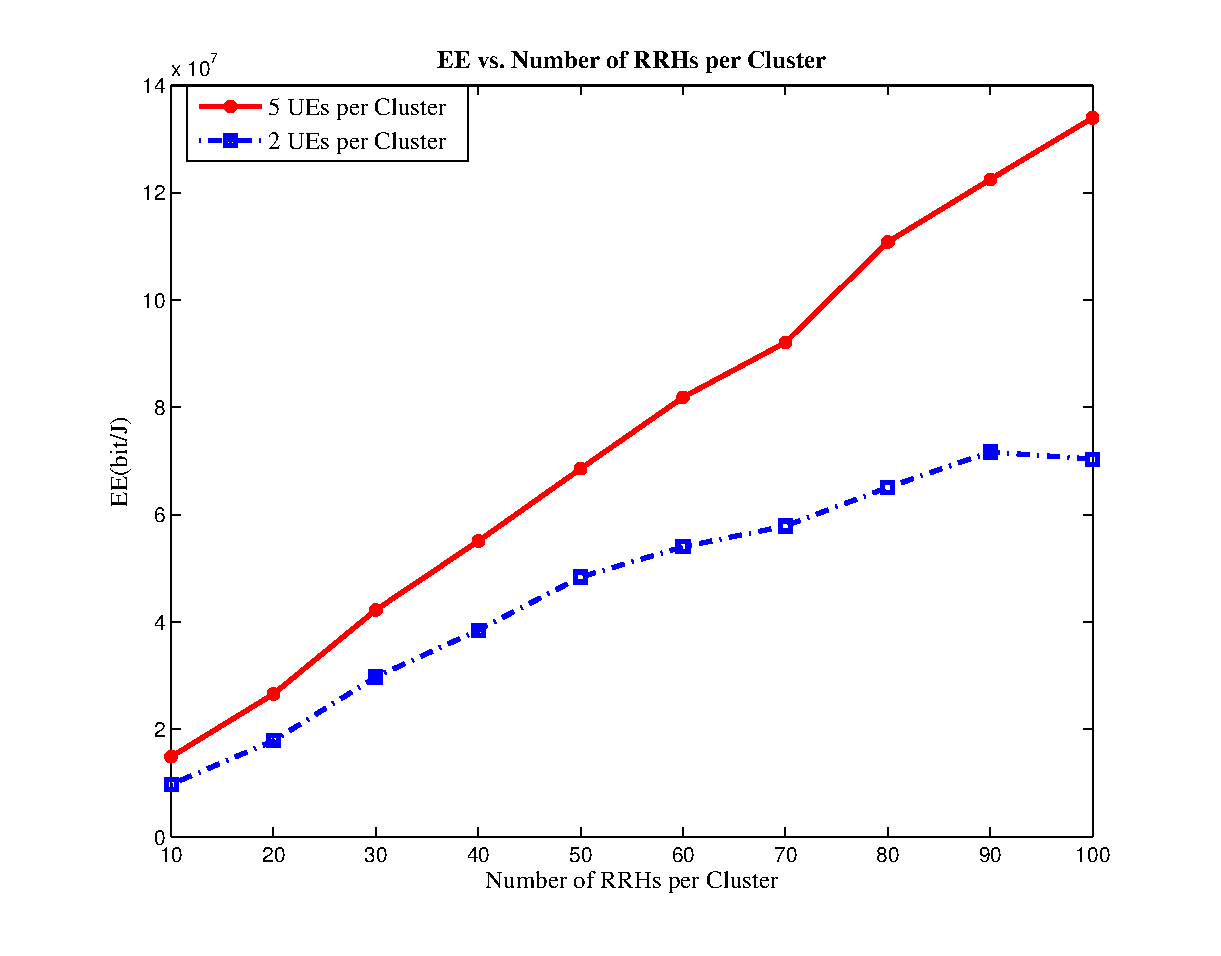
\includegraphics[width=\linewidth, height=12cm]{./fig3/rrh1}
  \caption{
  بازدهی انرژی با توجه به تغییرات تعداد واحدهای رادیویی  در هر خوشه برای توان بهینه برای 
   دو کاربر مختلف
   و پارامترهای جدول \ref{tab:title22}}
  \label{fig:nem1}
\end{figure}
 در شکل \ref{fig:nem1}، بازدهی انرژی سیستم \lr{MIMO C-RAN} بر اساس تعداد واحدهای رادیویی در هر خوشه برای مدل سیستم مورد نظر و برای دو تعداد کاربر متفاوت، رسم شده است. فرض اینجا بر این است که 2 خوشه برای لینک فروسو و دو خوشه برای فراسو وجود دارد.
 همانطور که  شکل  نشان می دهد، با افزایش تعداد واحدهای رادیوی، بازدهی انرژی افزایش می یابد زیرا  در اینجا با افزایش تعداد واحدهای رادیویی، مجموع توان کل افزایش می یابد در نتیجه نرخ انتقال داده نیز بیشتر می گردد و در نتیجه ی آن، بازدهی انرژی نیز افزایش یافته است. همچنین بازدهی انرژی برای تعداد کاربر بیشتر، به دلیل اینکه مجموع نرخ ها بیشتر می گردد، زیادتر می باشد.
 \begin{figure}[H]
  \centering
    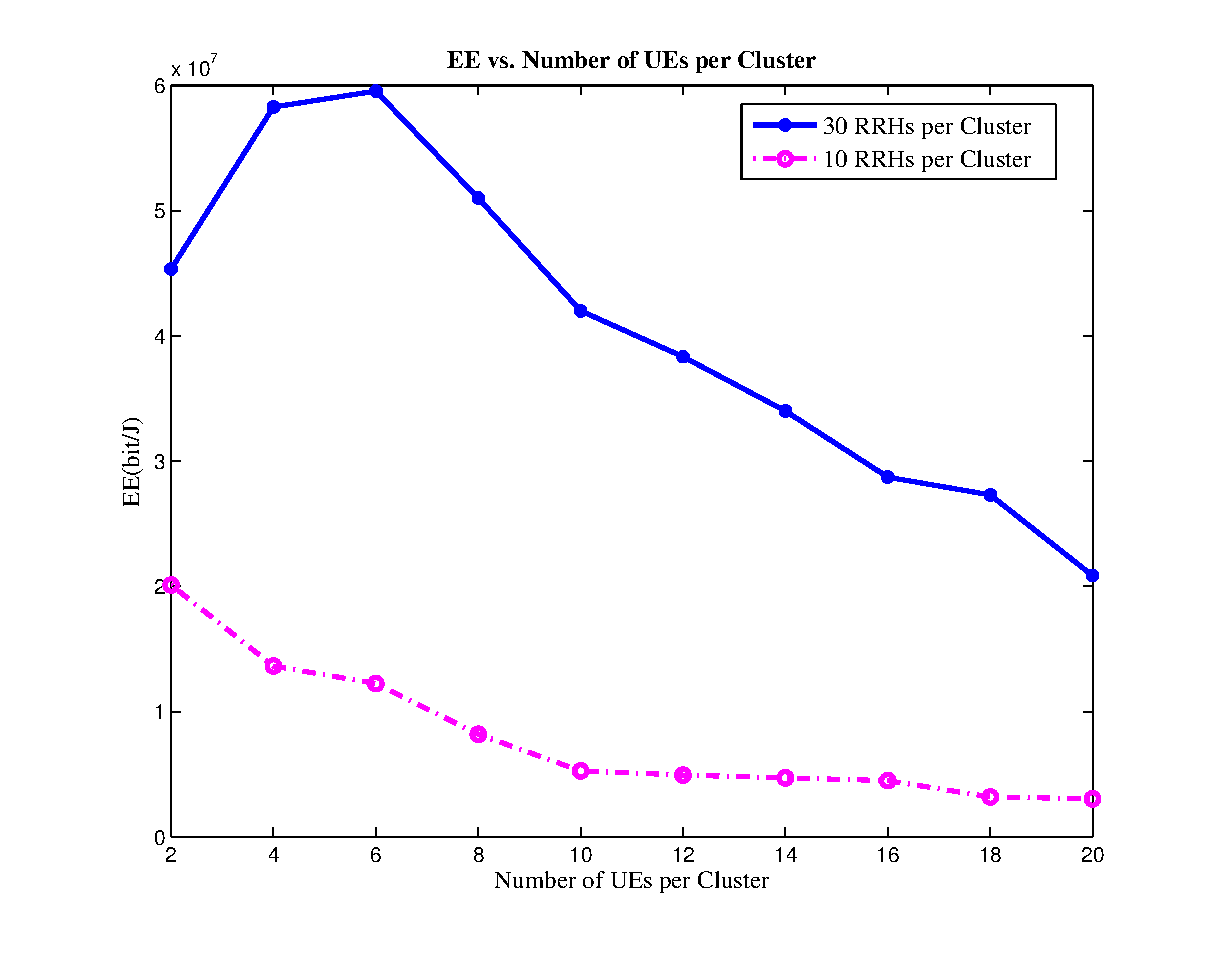
\includegraphics[width=\linewidth]{./fig3/ue4}
  \caption{  بازدهی انرژی با توجه به تغییرات تعداد کاربران در هر خوشه برای توان بهینه برای 
   دو واحد رادیویی مختلف
   و پارامترهای جدول
    \ref{tab:title22} }
  \label{fig:ue4}
\end{figure}

در شکل \ref{fig:ue4}، بازدهی انرژی بر اساس تعداد کاربران در هر خوشه برای مدل سیستم مورد نظر و برای دو تعداد واحد رادیویی متفاوت، رسم شده است. همانطور که  دیده می شود با افزایش تعداد کاربران، در حالتی که 30 واحد رادیویی در هر خوشه داریم، ابتدا به دلیل افزایش کاربران و افزایش مجموع نرخ ها، بازدهی انرژی زیاد شده و در نتیجه ی آن شیب نمودار زیاد می شود ولی از یک مقدار به بعد تداخل بین کاربران افزایش می یابد و منجر به کاهش بازدهی انرژی می گردد. زمانی که تعداد کاربران زیاد نیست، تداخل بین کاربران تاثیر کمی می گذارد و با افزایش کاربران بازدهی انرژی بهبود می یابد ولی زمانی که تعداد کاربران از حدی بیشتر می شود، میزان تداخل به قدری زیاد شده که نرخ انتقال داده کاهش یافته و در نتیجه ی آن، بازدهی انرژی کاهش می یابد. 
در حالتی که  10 واحد رادیویی در هر خوشه داریم، به دلیل اینکه میزان تداخل بین کاربران زیاد است و \lr{SINR} کم است، شیب نمودار از ابتدا منفی است و بازدهی انرژی کم می گردد.
 \begin{figure}[H]
  \centering
    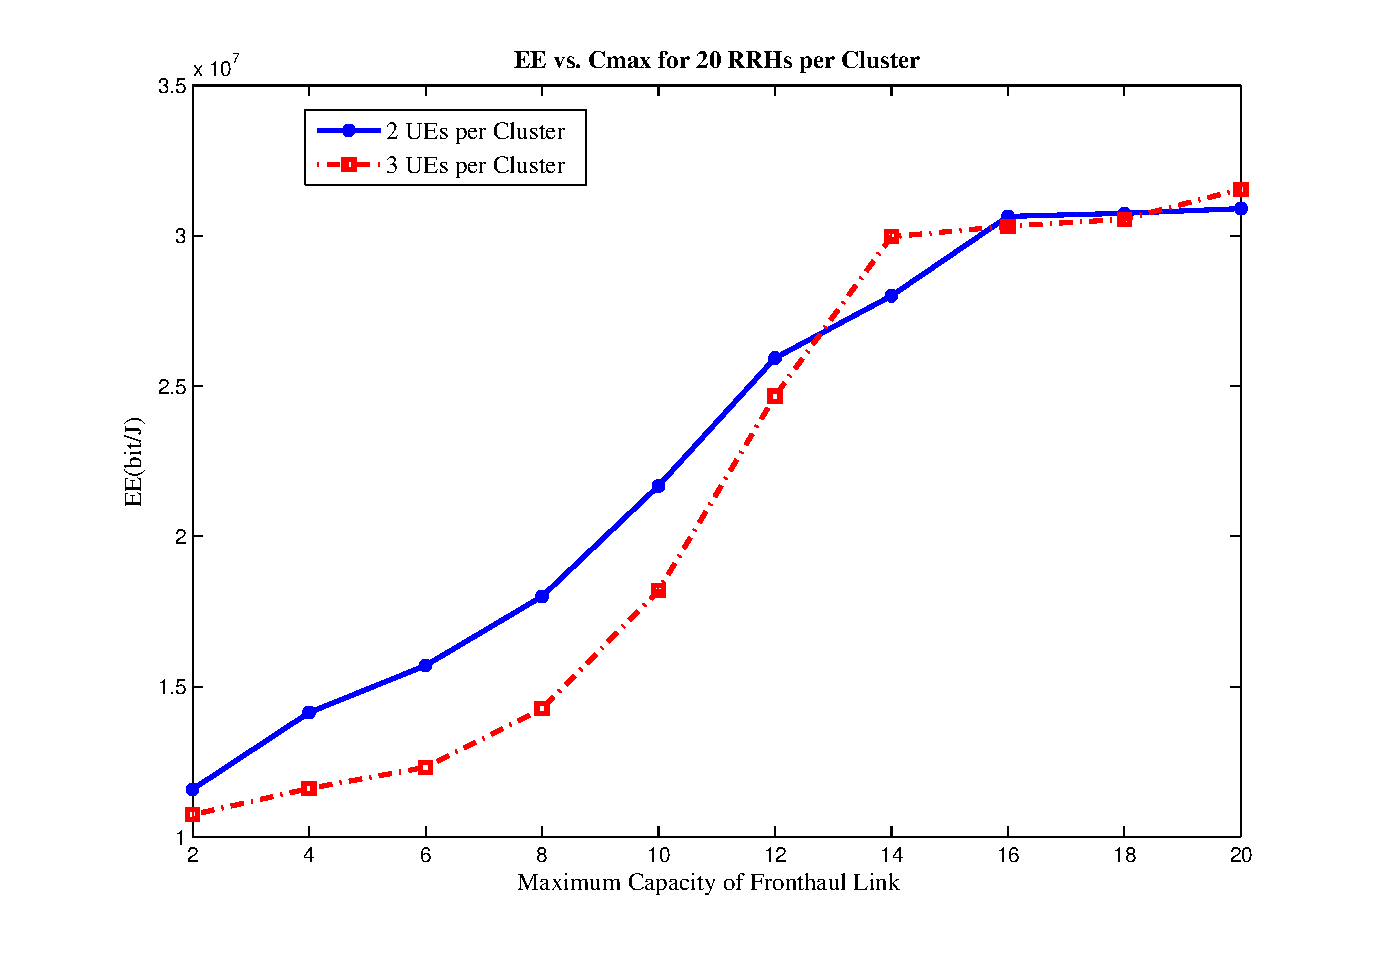
\includegraphics[width=\linewidth]{./fig3/c4}
  \caption{  
  بازدهی انرژی با توجه به تغییرات ظرفیت
   بیشینه ی لینک \lr{fronthaul}
   در هر خوشه برای توان بهینه برای 
   دو تعدا کاربر مختلف
   و پارامترهای جدول
    \ref{tab:title22} }
  \label{fig:c4}
\end{figure}
در شکل \ref{fig:c4}، بازدهی انرژی بر اساس تغییرات ظرفیت
   بیشینه ی لینک \lr{fronthaul} در هر خوشه برای مدل سیستم مورد نظر و برای دو تعداد کاربر متفاوت، رسم شده است.همانطور که  دیده می شود با افزایش این ظرفیت، بازدهی انرژی با شیب زیادی، افزایش یافته ولی از جایی به بعد شیب افزایش کم می گردد زیرا با افزایش بیشینه ی ظرفیت، تعداد بیت های بیشتری می تواند از این لینک عبور کند ولی از یک جایی به بعد، تعداد بیتهایی که در هر ثانیه وجود دارد از نرخ انتقال بیت کمتر است، پس با افزایش نرخ، بازدهی انرژی افزایش پیدا نمی کند. 
\section{نتیجه گیری}
در این فصل، مدل سیستم جدیدی که همزمان شامل چندین خوشه ی لینک فروسو و فراسو است، بیان شده است و همزمان مجموع نرخ های قابل دسترسی بر روی توان کل خوشه های لینک فراسو و فروسو بیشینه شده است و نمودارهای آن را بر حسب تعداد کاربران و واحدهای رادیویی رسم شده اند. با توجه به نمودارها، با افزایش تعداد واحدهای رادیویی توان ارسالی افزایش یافته و بازدهی انرژی بهبود می یابد.  همچنین با افزایش کاربران ابتدا بازدهی انرژی بهبود یافته زیرا مجموع توان افزایش می یابد ولی از حدی به بعد، تاثیر تداخل بین کاربران زیاد شده و بازدهی کاهش می یابد.
